\apendice{Especificación de Requisitos}

\section{Introducción}

Aunque este trabajo se centra sobre todo en investigación, cuando hablamos de requisitos nos referiremos a los de la aplicación Android generada. En esta sección se enumerarán los requisitos funcionales y no funcionales de la aplicación, y se definirán los casos de uso derivados.  

\section{Objetivos generales}

En la memoria se exponen los objetivos generales del trabajo, los cuales, dada la naturaleza del trabajo, se centran principalmente en la fase de investigación. En este apartado nos centraremos en los requisitos relativos al último de los objetivos generales expuestos: 

\begin{itemize}
	\item Investigar sobre técnicas del estado del arte aplicadas a problemas similares. 
	\item Aplicar técnicas de minería de datos siguiendo los pasos del Descubrimiento de Conocimiento en Bases de Datos (\textit{KDD})~\cite{fayyad1996data}.
	\item Explorar, aplicar y comparar distintas formas de preprocesado de los datos (filtrado, normalización, transformación, etc.). 
	\item Usar técnicas de proyección de datos a dos dimensiones para comprobar si los instancias de <<crisis>> son fácilmente separables de las instancias de <<no crisis>>. 
	\item Probar modelos de clasificación para conjuntos de datos con preprocesados basados en estadísticas simples.
	\item Probar modelos de clasificación para conjuntos de datos con preprocesados basados en características de series temporales.  
	\item Probar modelos de clasificación mediante \textit{ensembles} para conjuntos de datos desequilibrados. 
	\item Probar detección de anomalías mediante un modelo \textit{One-Class}.
	\item Comparar el rendimiento de los modelos obtenidos. 
	\item Comparar distintas métricas usadas para evaluar el rendimiento los modelos obtenidos. 
	\item Generar un modelo de clasificación capaz de detectar crisis epilépticas a partir de los datos disponibles. 
	\item \textbf{Desarrollar una app de Android para mostrar la aplicabilidad del modelo de clasificación generado.} 
\end{itemize}

\section{Catalogo de requisitos}

Aquí se enumeran los requisitos funcionales y no funcionales de la aplicación desarrollada para dispositivos Android. Dado que mi compañero de proyecto José Luis Garrido Labrador y yo hemos realizado dos aplicaciones (una web y una para Android) con el mismo objetivo y las mismas funcionalidades, la especificación de los requisitos  se ha realizado de forma conjunta, y por lo tanto, muchos de los puntos de estos apartados coincidirán en ambos trabajos. 

\subsection{Requisitos funcionales}
 
\begin{itemize}
	\item \textbf{RF-1 Confidencialidad del sistema:} Solamente los usuarios autorizados podrán acceder al sistema. 
	
\begin{itemize}
		\item \textbf{RF-1.1 Identificación de usuario:} los usuarios se identificarán con un \textit{nickname} y una contraseña 
		\item \textbf{RF-1.2 Rol de administración:} existirá un usuario especial que podrá administrar el sistema completamente sin restricciones.
		\item \textbf{RF-1.3 Visualización de una cama:} los usuarios validados deben poder observar los datos en tiempo real de las camas disponibles. 
		\item \textbf{RF-1.4 Restricción de acceso:} los usuarios solamente podrán tener acceso a los datos de las camas permitidas. 
		\item \textbf{RF-1.5 Acceso completo al administrador:} el administrador debe poder acceder a los datos de todas las camas existentes.
\end{itemize}
	
	\item \textbf{RF-2 Gestión de las camas:} El administrador debe poder gestionar las camas pudiendo añadir, modificar, borrar y dar acceso a un usuario a los datos de una cama determinada. 
	
\begin{itemize}
		\item \textbf{RF-2.1 Añadir cama:} el administrador debe poder añadir una nueva cama al sistema.
		\item \textbf{RF-2.2 Modificar cama:} el administrador debe poder modificar los datos una cama existente.
		\item \textbf{RF-2.3 Borrar cama:} el administrador debe poder borrar una cama del sistema.
		\item \textbf{RF-2.4 Asignar camas a usuarios:} el administrador se encarga de decidir qué usuario puede acceder a los datos de qué cama.
\end{itemize}
	
	\item \textbf{RF-3 Gestión de los usuarios:} el administrador debe poder gestionar los usuarios pudiendo añadir, modificar y borrar. El usuario debe poder gestionar su propia contraseña. 

\begin{itemize}
		\item \textbf{RF-3.1 Añadir usuario:} el administrador debe poder añadir un nuevo usuario al sistema.
		\item \textbf{RF-3.2 Modificar usuario:} el administrador debe poder modificar los datos un usuario existente. Igualmente el usuario debe poder modificar su propia contraseña. 
		\item \textbf{RF-3.3 Borrar usuario:} el administrador debe poder borrar un usuario del sistema.
\end{itemize}

	\item \textbf{RF-4 Visualización de los datos:} los usuarios deben poder ver, de las camas disponibles, el estado actual del paciente, la probabilidad de crisis epiléptica, sus constantes vitales y las presiones. 
	
\end{itemize}

\subsection{Requisitos no funcionales}

\begin{itemize}
	\item \textbf{RNF-1 Usabilidad:} la aplicación debe cumplir estándares de usabilidad teniendo una curva de aprendizaje baja y un uso de metáforas adecuado.
	\item \textbf{RNF-2 Confidencialidad:} los datos de las camas, al ser en parte constantes vitales de pacientes, solamente han de ser accesibles por los usuarios permitidos.
	\item \textbf{RNF-3 Escalabilidad:} el sistema debe ser escalable para adaptarse de manera correcta a un incremento de carga del sistema.
	\item \textbf{RNF-4 Seguridad:} los usuarios deben poder identificarse sólidamente con el sistema sin que sus datos o sus credenciales (\textit{tokens}) sean accesibles por terceros, incluso el administrador.
\end{itemize}


\section{Especificación de requisitos}

De la misma forma, en lo relativo a las funcionalidades del cliente, la especificación de los casos de uso se ha hecho de forma conjunta con mi compañero José Luis Garrido Labrador, por lo que los contenidos de este apartado coincidirán en gran medida con los suyos. 

\subsection{Actores}

En los casos de uso se distinguen dos actores: 
\begin{itemize}
	\item \textbf{Administrador:} Tiene acceso a la gestión de usuarios, la gestión de camas y la visualización de los datos de todas las camas existentes. 
	\item \textbf{Usuario:} Tiene acceso a la visualización de los datos de las camas que tiene asignadas y a la gestión de su propio usuario. 
\end{itemize}

\subsection{Diagramas de casos de uso}

\begin{figure}[H]
	\centering
	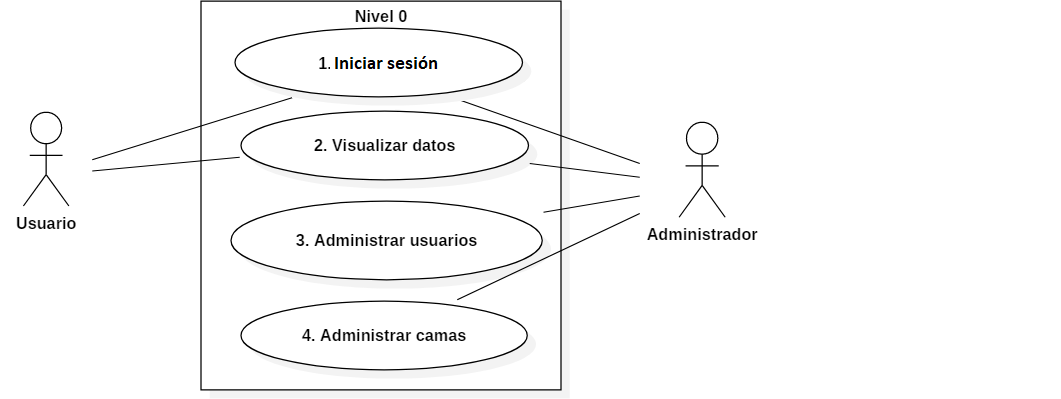
\includegraphics[width=1\textwidth]{../img/cu-n0.png}
	\caption{Diagrama de casos de uso, nivel 0.}
	\label{fig:cu-n0}
\end{figure}

\begin{figure}[H]
	\centering
	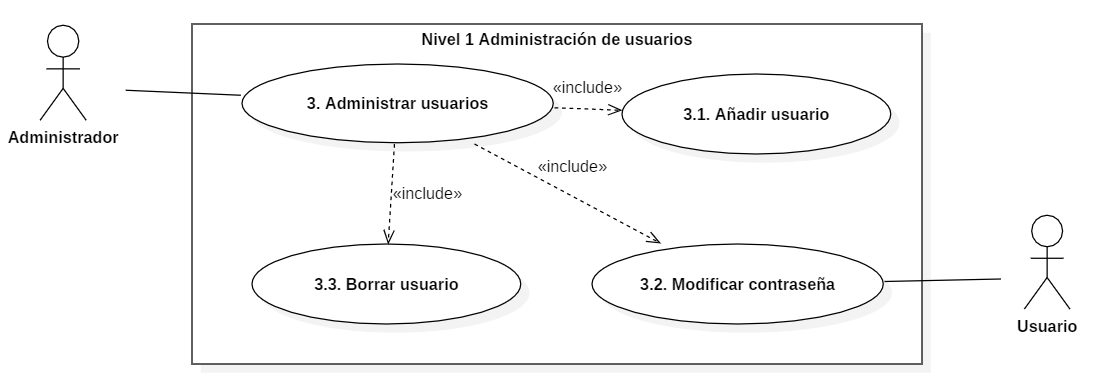
\includegraphics[width=1\textwidth]{../img/cu-n1-2.png}
	\caption{Diagrama de casos de uso, visualización de datos.}
	\label{fig:cu-n1.2}
\end{figure}

\begin{figure}[H]
	\centering
	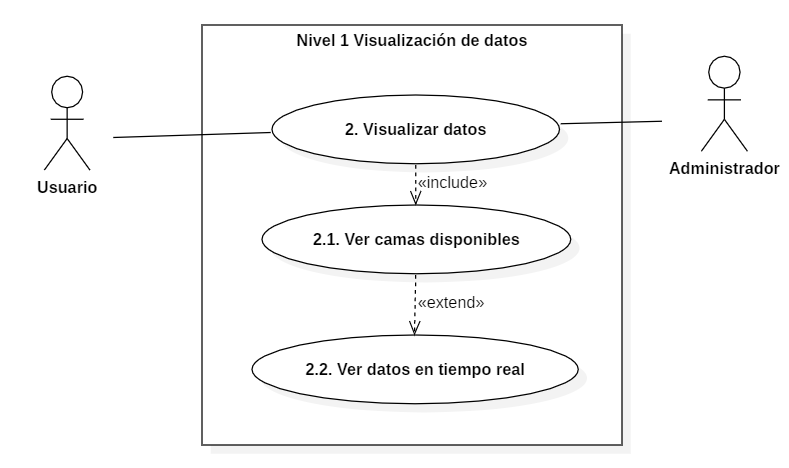
\includegraphics[width=1\textwidth]{../img/cu-n1-3.png}
	\caption{Diagrama de casos de uso, administración de usuarios.}
	\label{fig:cu-n1.3}
\end{figure}

\begin{figure}[H]
	\centering
	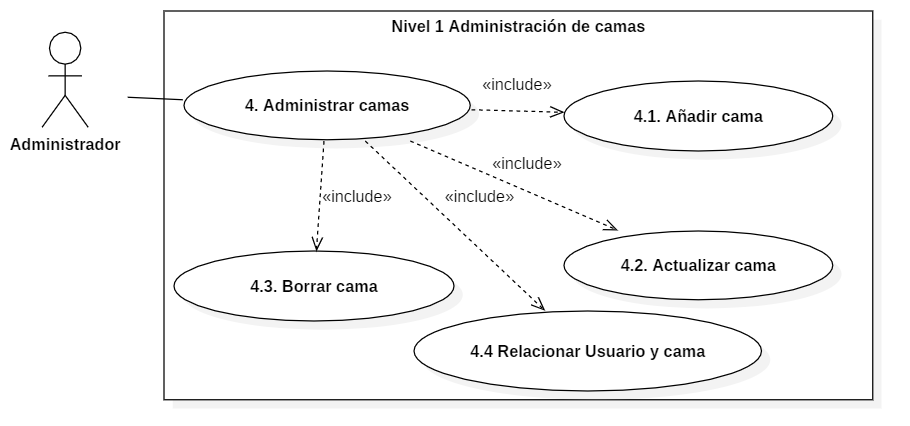
\includegraphics[width=1\textwidth]{../img/cu-n1-4.png}
	\caption{Diagrama de casos de uso, administración de camas.}
	\label{fig:cu-n1.4}
\end{figure}

\subsection{Especificación de casos de uso}

